\section{Qualitätsmessung der dekomprimierten Daten}
Bei verlustbehafteten Kompressionen muss die Qualität der dekomprimierten Daten sichergestellt werden. Im Verlauf der Arbeit wurden zwei Metriken verwendet: Die Standardabweichung und eine angepasste PSNR-HVS-M. Die Standardabweichung wird unabhängig von der Abtastrate berechnet und kann Subsampling Artefakte entdecken. Wie die Standardabweichung berechnet wird, ist im Abschnitt \ref{testsetup:ablauf} beschrieben.\\
Die PSNR-HVS-M wird für die Aufdeckung von Ringing Artefakten\cite{wiki:ringing:artefacts} berechnet. Ein Beispiel für Ringing Artefakte ist in der Abbildung \ref{resultate:loesung1:dct:randbehandlung:jvhartefakte} im Abschnitt \ref{resultate:loesung1:ringing} zu sehen. Die PSNR-HVS-M stammt aus der Bildverarbeitung. Das Ziel des Fehlermasses ist es, eine hohe Korrelation zwischen der Metrik und dem menschlichen Augenmass zu erreichen. Wie die PSNR-HVS-M Metrik angepasst und umgesetzt wurde, ist im Abschnitt \ref{testsetup:psnr} beschrieben.\\
Für die Messungen wurden spezielle Aufnahmen der Feldlinien gewählt. Wie die Aufnahmen ausgewählt wurden, ist im Abschnitt \ref{testsetup:auswahl_erhebung} beschrieben.

\subsection{Auswahl und Erhebung der Testdaten}\label{testsetup:auswahl_erhebung}
Die Testdaten sollen zu einem alle Randfälle abdecken, als auch durchschnittliche Fälle enthalten. Aus diesem Grund wurden insgesamt zehn Datensätze ausgewählt: Vier Datensätze mit hoher Sonnenaktivität, zwei mit wenig und vier zufällig. Für die vier Datensätzen mit hoher Aktivität wurde in den Jahren 2014 und 2013 nach den grössten Solare Flares gesucht. Für die Datensätze mit wenig Aktivität wurde nach Zeiträumen mit möglichst kleinen Solar Flares gesucht.\\
Die Feldlinien werdenalle sechs Stunden berechnet und Solar Flares sind spontane Ereignisse. Für die Solar Flares wurde deshalb beachtet, dass die Datensätze vor dem Ereignis verwendet wurden. Grosse Solar Flares entladen das Magnetfeld der Sonne. Vor dem Ereignis ist das Magnetfeld komplex.\\
[\baselineskip]
Wie im Abschnitt \ref{konzept:ist-komprimierung} beschrieben, wird bereits eine einfache verlustbehaftete Kompression Simulation. Für die Testdaten wurde diese entfernt, was die rohe Datenmenge entsprechend anwachsen liess auf etwa 10 MiBytes pro Aufnahme.

\subsection{Berechnung der Standardabweichung}\label{testsetup:ablauf}
Die dekomprimierte Linie ähnelt dem Original, wenn die Abweichungen konstant bleiben. Für diesen Fall wurde Die Standardabweichung ausgewählt. Die originale und dekomprimierte Feldlinie können unterschiedliche Abtastraten aufweisen. Die Standardabweichung muss deshalb unabhängig von der Abtastrate berechnet werden.\\
\begin{figure}[!htbp]
	\center
	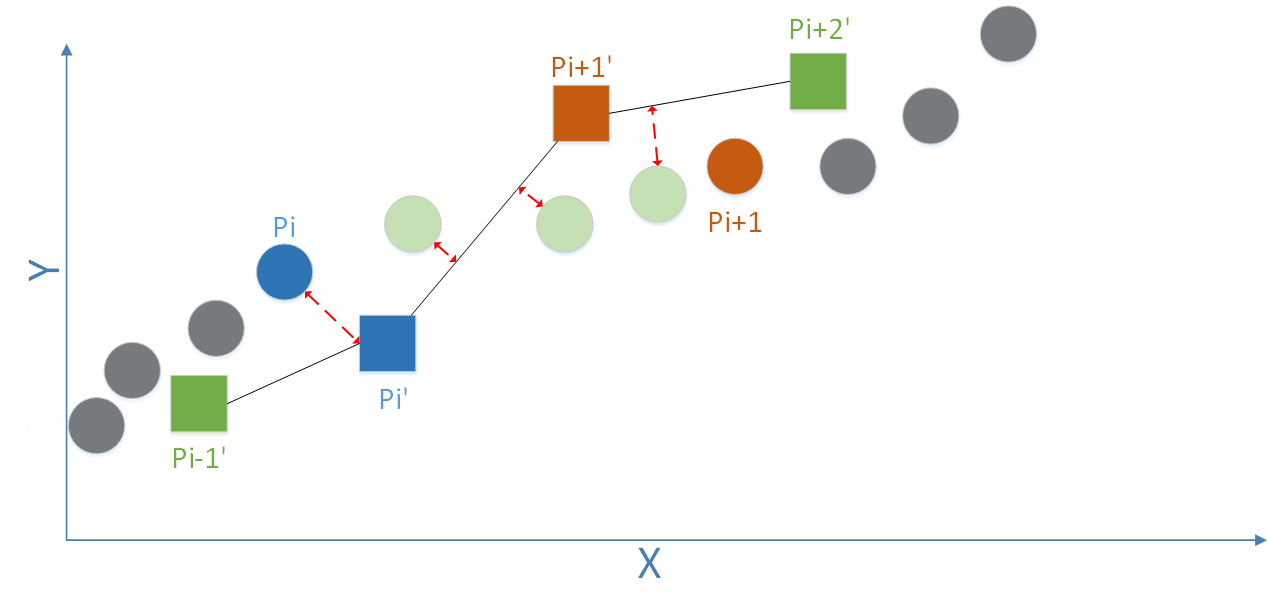
\includegraphics[width=0.9\textwidth,height=7cm,keepaspectratio]{./pictures/testsetup/errorcalc.png}
	\caption{Darstellung der Fehlerberechnung. Die Punkte sind die Originaldaten, die Quadrate sind die Punkte nach der Kompression.}
	\label{testsetup:ablauf:fehlerberechnung:diagramm}
\end{figure} 
Um die Abweichung zu berechnen wird konzeptionell zwischen die dekomprimierten Punkte eine Linie gezogen und den Abstand zwischen dieser Linie und den Originalpunkte berechnet. Der Vorgang ist dargestellt im Diagramm der Abbildung \ref{testsetup:ablauf:fehlerberechnung:diagramm}. Für jeden Punkt $P_i'$ aus den dekomprimierten Punkten $D$, nehme $P_i'$, $P_{i-1}'$,$P_{i+1}'$ und $P_{i+2}'$. Ziehe drei Strecken, von $P_{i-1}'P_i'$, $P_{i}'P_{i+1}'$ und $P_{i+1}'P_{i+2}'$. Suche von $P_i'$ den Originalpunkt $P_i$ aus allen Originalpunkten $O$, berechne den minimalen Abstand zu den drei Strecken. Führe das für alle folgenden Originalpunkte durch, bis $P_{i+1}$ erreicht wurde.\\
[\baselineskip]
Die Abstandsberechnung von Strecke $s$ zu einem Punkt $P$ erfolgt in zwei Schritten: Zuerst wird mit der Formel \eqref{testsetup:ablauf:formula:on_line} überprüft, ob eine Senkrechte durch $P$ auf der Strecke $s$ zu liegen kommt. Falls das der Fall ist, wird der Abstand von $P$ zu $s$ berechnet \eqref{testsetup:ablauf:formula:distance}. Falls nicht, wird die kürzeste Distanz der Eckpunkte der Strecke zu $P$ berechnet.\\
\begin{equation} \label{testsetup:ablauf:formula:on_line}
 t = \frac{\vec{AB}*\vec{AP}}{\lvert \vec{AB}\rvert ^2} \quad 0 \leq t \leq 1
\end{equation}
\begin{equation}\label{testsetup:ablauf:formula:distance}
distance = \frac{\lvert \vec{BA}\times \vec{BP}\rvert}{\lvert \vec{BP} \rvert}
\end{equation}
$A$ und $B$ sind die Eckpunkte der Strecke. Falls $0 \leq t \leq 1$, existiert eine Senkrechte durch $P$ mit Fusspunkt auf der Strecke $s$. Die Distanz von $P$ zu $s$ wird mit der Formel \eqref{testsetup:ablauf:formula:distance} berechnet.\\
Wenn das nicht möglich ist, wird der kürzere Distanz von $P$ zu einem der Eckpunkte genommen. 

\subsubsection{Berechnung der Standardabweichung}
\begin{equation} \label{testsetup:ablauf:formula:deviation}
	\begin{split}
		\sigma(X)& = \sqrt{variance(X)}\\
		variance(X) & = \sum{(x_i - E(x_i))^2}
	\end{split}
\end{equation}
Die Standardabweichung $\sigma$ einer Beobachtungsreihe $X$ $(x_1,x_2,x_3,\ldots, x_n-1)$ ergibt sich aus der Wurzel der Varianz von $X$. Die Varianz von $X$ kann errechnet werden, wenn man den Distanz jeder Beobachtung $x_i$ mit dem Erwartungswert $E(x_i)$ berechnet und quadriert. Die Beobachtung ist im diesen Fall ein Punkt der dekomprimierten Linie, während der Erwartungswert der Originalpunkt ist. Die Distanz wird mit dem besprochnen Verfahren \ref{testsetup:ablauf} berechnet. Die Summe der quadratischen Abstände ergibt die Varianz. Die Varianz wird über alle Testdaten berechnet, somit erhält man für einen Test einen Wert für die Standardabweichung.

\subsection{Berechnung der angepassten PSNR-HVS-M}\label{testsetup:psnr}
Die Peak-Signal-Noise-Ratio (PSNR) Metrik ist ein weitverbreitetes Fehlermass in der Bildverarbeitung. Es wird für die Messung des Fehlers zwischen dekomprimierten Bild und dem Original eingesetzt. 
\begin{equation} \label{testsetup:psnr:formula:psnr}
\begin{split}
PSNR & = 20 * log_{10}(MAX_I) - 10*log_{10}(MSE) \\
MSE & = \frac{1}{n}\sum_{i=0}^{N-1}[E(i)-D(i)]^2
\end{split}
\end{equation}
Die PSNR \eqref{testsetup:psnr:formula:psnr} besteht aus dem maximal möglichen Wert $MAX_I$ und dem ''Mean Squared Error´´ ($MSE$). Wobei $E()$ die Originaldaten und $D()$ die verzerrten Daten darstellen. Das Problem der PSNR ist, dass sie nicht mit der menschlichen Wahrnehmung übereinstimmt. Ponomarenko et al.  \cite{ponomarenko2007between:psnr} haben eine modifizierte PSNR entwickelt; die PSNR Human Visual System Masking (HVS-M). In ihren Messungen erreichten sie eine hohe Korrelation zwischen menschlicher Wahrnehmung von verzerrten Bildern und dem neuen Fehlermass.

Der Unterschied zwischen der PSNR und der PSNR-HVS-M liegt in der Berechnung des durchschnittlichen quadratischen Fehlers. Das Diagramm der Abbildung \ref{testsetup:ablauf:psnr:flowchart} zeigt den Ablauf der neuen Berechnung.\\
\begin{figure}[!htbp]
	\center
	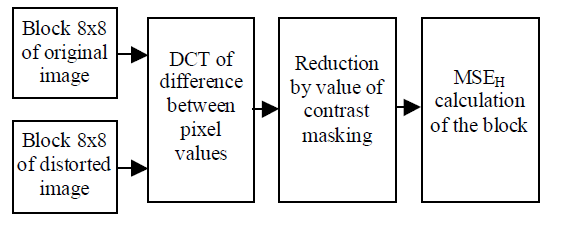
\includegraphics[width=0.8\textwidth,height=3.5cm,keepaspectratio]{./pictures/testsetup/psnr-hvs-m-flow.png}
	\caption{Flussdiagramm der PSNR-HVS-M Berechnung \cite{ponomarenko2007between:psnr}.}
	\label{testsetup:ablauf:psnr:flowchart}
\end{figure}
PSNR-HVS-M berechnet die Differenz zwischen dem Originalbild $E$ und dem verrauschtem Bild $D$ und führt die Daten mittels einer DCT in den Frequenzraum. Der nächste Schritt Contrast Maskin reduziert die Differenz, wenn das menschliche Auge den Frequenzunterschied nicht erkennen kann. Aus den $MSE_H$ Werten wird mit der Formel \eqref{testsetup:psnr:formula:psnr} die PSNR-HVS-M berechnet.

\subsubsection{Contrast Masking}
Um das Contrast Masking zu berechnen, führt Ponomarenko et al. die gewichtete Energie der DCT Koeffizienten $E_w$ \eqref{testsetup:psnr:formula:weighted_energy}und den masking effect $E_m$ \eqref{testsetup:psnr:formula:masking_effect} ein:\\
\begin{equation}\label{testsetup:psnr:formula:weighted_energy}
 E_w(X)  = \sum_{i=0}^{7}\sum_{j=0}^{7}[X_{ij}]^2 C_{ij}
\end{equation}
\begin{equation} \label{testsetup:psnr:formula:masking_effect}
	E_m(X)  = \frac{1}{f_m}E_w(X)
\end{equation}
Wobei $X$ die Kosinus-Koeffizienten eines $8*8$ Bildblocks sind und $C$ die Gewichtungen der Frequenzen. Der Normalisierungsfaktor $f_m$ wurde experimentell ermittelt und auf $16$ festgelegt. Ponomarenko et al. argumentiert, dass der Unterschied zwischen einem Block $X_e$ und einem verrauschten Block $X_d$ unsichtbar sind, wenn die Formel \eqref{testsetup:psnr:formula:masking} erfüllt ist.
\begin{equation} \label{testsetup:psnr:formula:masking}
	E_w(X_e-X_d) < max[E_m(X_e),E_m(X_d)]
\end{equation}
Die Eigenschaft der Ungleichung \eqref{testsetup:psnr:formula:masking} fliesst mit der Formel \eqref{testsetup:psnr:formula:error} in die Distanzberechnung ein.
\begin{equation} \label{testsetup:psnr:formula:error}
	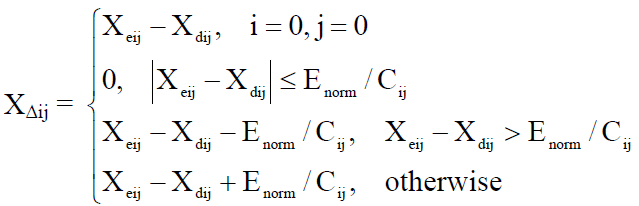
\includegraphics[scale=0.5]{./pictures/testsetup/mseH}\\
\end{equation}
Wobei $E_{norm} = \sqrt{max[E_m(X_e),E_m(X_d)] / 64}$. $X_{eij}$ ist der DCT Koeffizient des Originalblockes und $X_{dij}$ der Koeffizient des verrauschten Blockes. Dabei ist es irrelevant ob die DCT Koeffizienten subtrahiert oder wie in der Abbildung \ref{testsetup:ablauf:psnr:flowchart} angedeutet, zuerst die Differenz der Pixelwerte berechnet und diese DC transformiert werden.

Wie gut die PSNR-HVS-M Metrik mit dem menschlichen Auge übereinstimmt, hängt vom Normalisierungsfaktor $f_m$ und von der Wahl der Gewichtungen $C$ ab. Ponomarenko et al. verwendeten die normalisierten ($\frac{10}{x}$) und quadrierten Werte der JPEG/JFIF Quantisierungsmatrix \cite{wallace1992jpeg}. Es ist zu beachten, dass der DC-Koeffizient\cite{wiki:dccoeff} nicht im Contrast Masking berücksichtigt wird, für den Wert wird die normale PSNR berechnet. Der DC-Koeffizient stellt die durchschnittliche Helligkeit in einem Block dar. Das menschliche Auge kann auch kleine Unterschiede in dieser Frequenz erkennen.

\subsubsection{Umsetzung und Anpassung der PSNR-HVS-M für diese Arbeit}
Der grösste Unterschied zur Arbeit von Ponomarenko et. al. ist der Einbezug des DC-Koeffizienten ins Contrast-Masking. Der DC-Koeffizient repräsentiert bei den Feldlinien eine Verschiebung. Das menschliche Auge kann leichte Verschiebungen der Feldlinien kaum unterscheiden. Des Weiteren musste für die Feldlinie eine eigene Quantisierungsmatrix gefunden werden, aus denen die Gewichtungen berechnet werden. Es wurde eine DCT-Kompression entwickelt, welche keine sichtbaren Artefakte aufweist. Die Quantisierungsmatrix wurde übernommen und auf dieselbe Weise normalisiert.\\
Für die PSNR wird der maximale Wert $MAX_I$ benötigt. Hier wurde der maximal mögliche Wert der PFSS Simulation verwendet, den vierfachen Sonnenradius.

Der letzte Wert, den es zu setzen gibt, ist der Normalisierungsfaktor $f_m$. Ponomarenko et. al. schrieb keine zusätzliche Information oder Begründung zu diesem Wert. Dieser Wert stellt ein, wie stark das Contrast-Masking einfliessen soll. Je höher der Wert ist, desto ähnlicher ist die PSNR-HVS-M Metrik der normalen PSNR.\\
Die Tabelle \ref{testsetup:psnr:umsetzung:tabelle:f_m} erforscht den Einfluss des $f_m$ Faktors. Dazu wurde die PSNR-HVS-M zu drei dekomprimierten Simulationen berechnet, welche eine unterschiedliche Qualität aufweisen.

\begin{table}[!htbp]
\center
\begin{tabular}{r|c|c|c}
	Qualität &$f_m$ 8 &$f_m$ 16 &$f_m$ 32 \\\hline
	Keine sichtbare Artefakte & 96.8 dB & \textbf{95.6} dB& 94.5 dB \\
	Kaum sichtbare Artefakte & 95.8 dB & \textbf{94.4} dB& 93.3 dB\\
  Sichtbare Artefakte & 90.0 dB & \textbf{88.3} dB & 87,0 dB
\end{tabular}
\caption{Einfluss des $f_m$ Faktors auf die PSNR-HVS-M.}
\label{testsetup:psnr:umsetzung:tabelle:f_m}
\end{table}
Für diesen Anwendungsfall scheint der Faktor $f_m$ sich stabil zu verhalten: der Faktor kann verdoppelt oder halbiert werden und die resultierenden Distanzen bleiben in derselben Grössenordnung. Es wurde der Standardwert von $16$ übernommen. Eine Anpassung von $f_m$ scheint nicht die Metrik massgebend zu verändern und hat vermutlich weniger Einfluss als die Gewichtung der DCT Koeffizienten.

Die PSNR-HVS-M ist nicht unabhängig von der Abtastrate. Für diese Arbeit werden die Originaldaten auf dieselbe Punktmenge reduziert. Wenn pro Feldlinie genau ein Punkt exakt abgespeichert wird, würde die PSNR-HVS-M trotzdem eine hohe Ähnlichkeit zwischen Original und dekomprimierten Feldlinien ergeben. Dies ist Vertretbar, da die Standardabweichung diesen Fall abdeckt und eine hohe Distanz ausgeben wird. Die PSNR-HVS-M soll hauptsächlich Artefakte aufdecken, welche in der Standardabweichung nicht ins Gewicht fallen wie die Ringing Artefakte aus Abschnitt \ref{resultate:loesung1:ringing}.